\section{Linear Quadratic Regulator} \label{sec:lqr}
The first design approach is obtained using a LQR. First, a state space model of the system is created based on the equations derived in \autoref{chap:model}. Then, a cost function based on the state errors and the input usage is minimized in order to calculate the controller gains. 

\subsection{State Space Model}
The linearized model derived in \autoref{sec:linearizationModel}, consisting of \autoref{eq:x_pos_model_lin} to \ref{eq:psi_model_lin}, needs to be represented in state space form to design a state space controller. In order to do that, the three degrees of freedom model used for the control of the vessel is represented as
\begin{flalign}
    \vec{\dot{x}}(t) &= \vec{A} \vec{x}(t) + \vec{B} \vec{u}(t)  \ ,
    \label{xDotLinear}\\
    \vec{y}(t) &= \vec{C} \vec{x}(t) + \vec{D} \vec{u}(t) \ .
    \label{yLinear} 
\end{flalign}
\begin{where}
    \va{\vec{x}}{is the state vector}{}
    \va{\vec{u}}{is the input vector}{}
    \va{\vec{y}}{is the output vector}{}
    \va{\vec{A}}{is the state matrix}{}
    \va{\vec{B}}{is the input matrix}{}
    \va{\vec{C}}{is the output matrix}{}
    \va{\vec{D}}{is the feedforward matrix}{}
\end{where}

The state vector is constituted by the angle and angular velocity in yaw as well as the velocity in $x_\mathrm{b}$. The system outputs are the yaw angle and velocity in $x_\mathrm{b}$. The input vector is composed of the two forces applied in the body frame.
 
\begin{minipage}{0.32\linewidth}
    \begin{flalign}
        \vec{x(t)} = 
        \begin{bmatrix}
            \psi\\
            \dot{\psi}\\
            \dot{x}_{b} \\
        \end{bmatrix} \nonumber
        \label{xVector} \ ,
    \end{flalign}  
\end{minipage}\hfill
%\hspace{0.03\linewidth}
\begin{minipage}{0.32\linewidth}
    \begin{flalign}
        \vec{y(t)} = 
        \begin{bmatrix}
            \psi \\
            \dot{x}_{b} \\
        \end{bmatrix} \nonumber
        \label{yVector}  \ ,
    \end{flalign}
\end{minipage}\hfill
%\hspace{0.03\linewidth}
\begin{minipage}{0.32\linewidth}
    \begin{flalign}
        \vec{u(t)}= 
        \begin{bmatrix}
            F_1 \\
            F_2 
        \end{bmatrix}
        \label{uVector} \ .
    \end{flalign} \nonumber
\end{minipage}\hfill

The resulting $\vec{A}$, $\vec{B}$, $\vec{C}$ and $\vec{D}$ matrices are
\begin{flalign}
    \vec{A} &=
    \begin{bmatrix}
        \ 0 & 1                   & 0                \ \ \ \\ 
        \ 0 & -\frac{d_\psi}{I_\mathrm{z}} & 0                \ \ \ \\ 
        \ 0 & 0                   & -\frac{d_\mathrm{x}}{m} \ \ \     
    \end{bmatrix} \ ,\rule{30px}{0px}
    \vec{B} = 
    \begin{bmatrix}
        \ 0               & 0                \ \ \ \\
        \ \frac{l_1}{I_\mathrm{z}} & -\frac{l_2}{I_\mathrm{z}} \ \ \ \\   
        \ \frac{1}{m}   & \frac{1}{m}    \ \ \
    \end{bmatrix} \ ,\rule{30px}{0px}
    \vec{C} =   
    \begin{bmatrix}
        \ 1 & 0 & 0  \ \ \ \\ 
        \ 0 & 0 & 1  \ \ \    
    \end{bmatrix} \ ,
    \label{eqStateSpaceABC}
\end{flalign}
while, as for most mechanical systems, the $\vec{D}$ matrix is zero.

\subsection{Controller Design}
The design in carried out in the discrete domain. To do so, it is necessary to discretize the system. A discrete state space model is expressed as,
%
\begin{flalign}
  \vec{x}(k+1) &= \vec{A}_\mathrm{z} \vec{x}(k) + \vec{B}_\mathrm{z} \vec{u}(k)
  \label{xDotLinearDiscrete} \ ,\\
  \vec{y}(k)   &= \vec{C}_\mathrm{z} \vec{x}(k) + \vec{D}_\mathrm{z} \vec{u}(k) \ ,
  \label{yLinearDiscrete} 
\end{flalign}
%
where the z subindexes indicate the matrices being discrete and $k$ is the sample index.

The model is discretized using the zero order hold method, as it does not introduce a $\vec{D}_\mathrm{z}$ matrix, with a sampling time, $T_s = 0.05$ s. This sampling time is suitable as it is faster than the system's dynamics, which ensures the controller is able to react faster to changes in the system. In \autoref{fig:discreteSSBlock} the discrete system is shown in a block diagram.
%
\begin{figure}[H]
  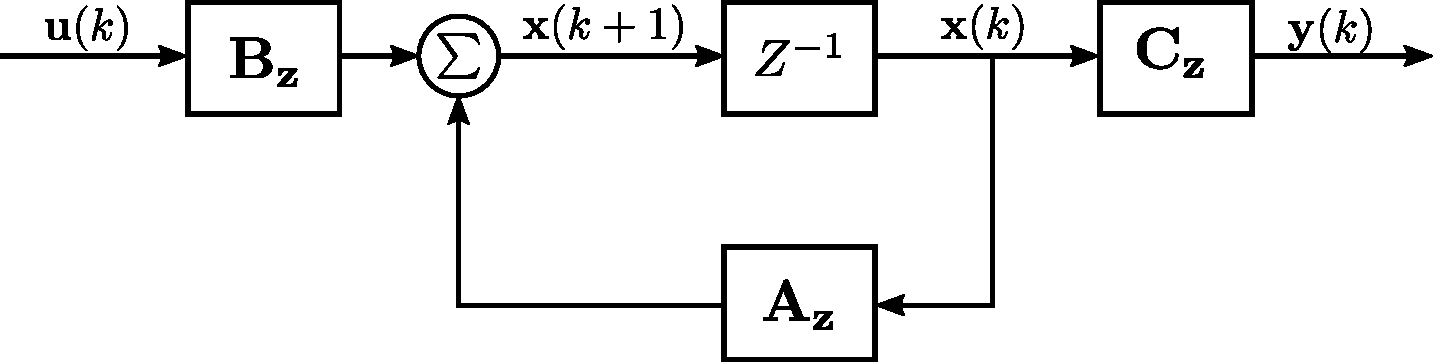
\includegraphics[width=0.6\textwidth]{figures/discreteSystemBlockDiagram}
  \caption{Block diagram of the discrete system.}
  \label{fig:discreteSSBlock}
\end{figure}
%
In order to track a reference and handle input disturbances, it is chosen to also include integral action in the design. The final control structure is seen in \autoref{fig:blockConrolDesignLQR}.
%
\begin{figure}[H]
  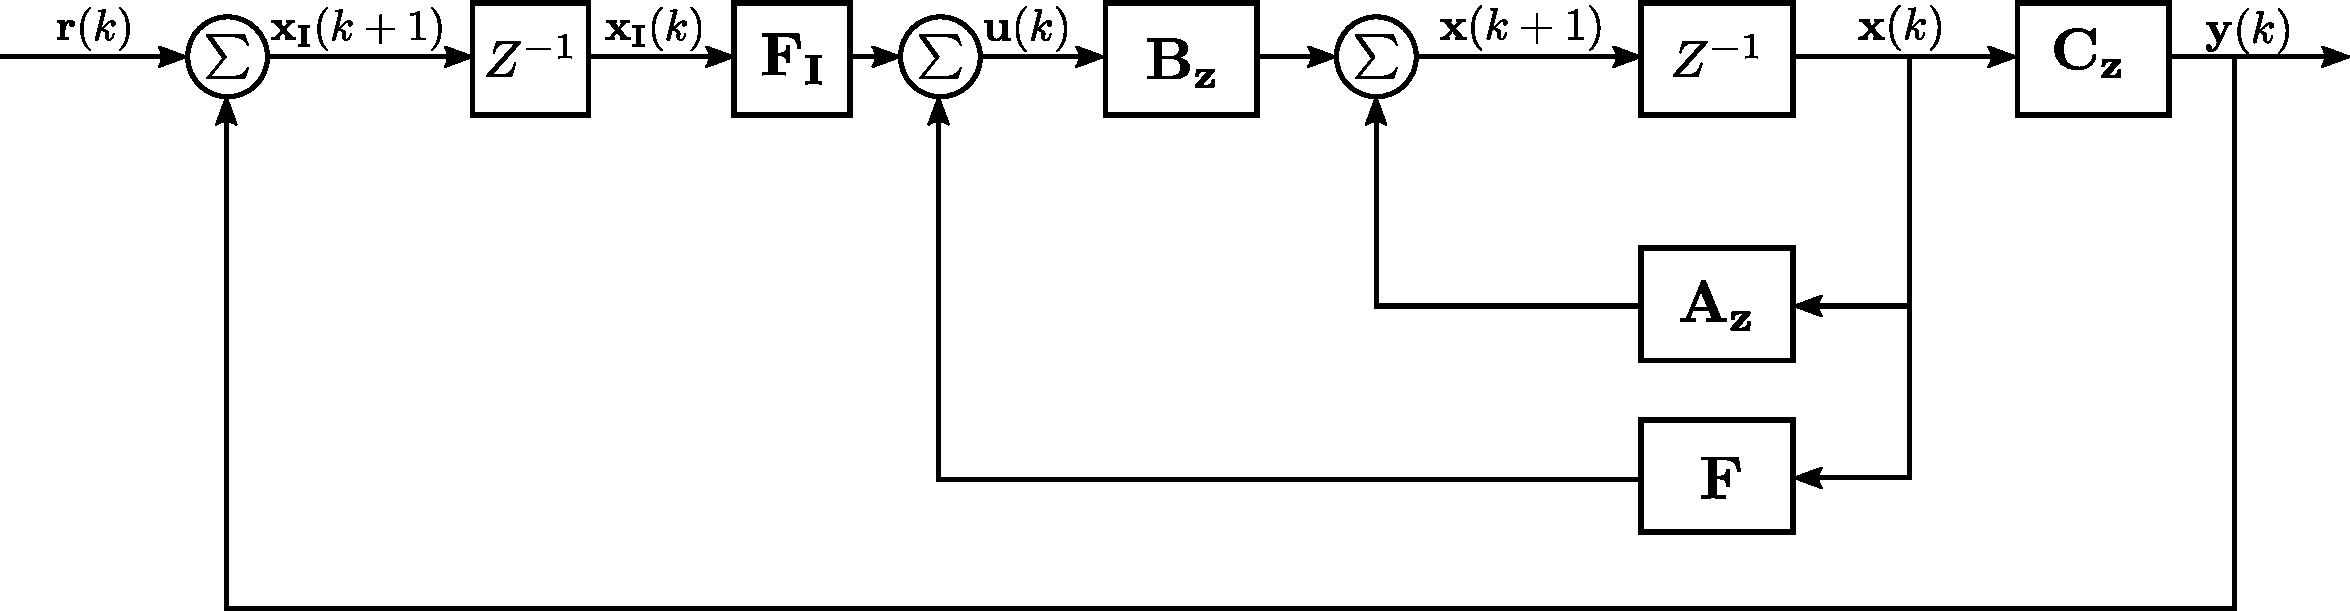
\includegraphics[width=0.9\textwidth]{figures/integralControlBlockDiagram}
  \caption{Block diagram of the control structure in the discrete domain. $\vec{F}$ correspond to the feedback gain matrix while $\vec{F}_\mathrm{I}$ is the integral gain matrix.}
  \label{fig:blockConrolDesignLQR}
\end{figure}

To design this system, it is convenient to express it on the following form
%
\begin{flalign}
  \vec{x}_\mathrm{e}(k+1) &= \vec{A}_\mathrm{e} \vec{x}_\mathrm{e}(k) + \vec{B}_\mathrm{e} \vec{u}(k) + \vec{r}(k)
  \label{eq:xDotLinearDiscrete} \ ,\\
  \vec{y}(k)     &= \vec{C}_\mathrm{e} \vec{x}_\mathrm{e}(k) \ .
  \label{eq:yLinearDiscrete} 
\end{flalign}
where the subindex "e" denotes the extended system.

To describe the control design in this form, the $\vec{A}_\mathrm{e}$, $\vec{B}_\mathrm{e}$ and $\vec{C}_\mathrm{e}$ matrices must be constructed. From \autoref{fig:blockConrolDesignLQR}, the discrete state space model for the integral is derived and shown in \autoref{eq:xIDiscrete}.
%
\begin{flalign}
  \vec{x}_\mathrm{I}(k+1) &= \vec{x}_\mathrm{I}(k) + \vec{y}(k) + \vec{r}(k) \ , \label{eq:xIDiscrete1}  \\
  \vec{x_I}(k+1) &= \vec{x}_\mathrm{I}(k) - C_\mathrm{z} \vec{x}_\mathrm{I}(k) + \vec{r}(k) \ .
  \label{eq:xIDiscrete}
\end{flalign}
where the subindex "I" stands for integral .

This leads to the discrete state space model extended with the integral states expressed as
%
\begin{flalign}
  \begin{bmatrix}
    \vec{x}(k+1)  \\
    \vec{x}_\mathrm{I}(k+1)
  \end{bmatrix}
  &=
  \begin{bmatrix}
    \vec{A}_\mathrm{z,3x3} & \vec{0}_\mathrm{3x2} \\
   -\vec{C}_\mathrm{z,2x3} & \vec{I}_\mathrm{2x2} \\
  \end{bmatrix}
  \begin{bmatrix}
    \vec{x}(k)    \\
    \vec{x}_\mathrm{I}(k)
  \end{bmatrix}
  +
  \begin{bmatrix}
    \vec{B}_\mathrm{z,3x2} \\
    \vec{0}_\mathrm{2x2}
  \end{bmatrix}
  \vec{u}(k)
  +
  \begin{bmatrix}
    \vec{0}_\mathrm{3x2} \\
    \vec{I}_\mathrm{2x2}
  \end{bmatrix}
  \vec{r}(k) \ ,
  \label{eq:discreteSSWithIntegralX} \\
  \vec{y}(k)
  &=
  \begin{bmatrix}
    \vec{C}_\mathrm{z,2x3} &  \vec{0}_\mathrm{2x2}
  \end{bmatrix}
  \begin{bmatrix}
    \vec{x}(k)    \\
    \vec{x}_\mathrm{I}(k)
  \end{bmatrix}  \ ,
  \label{eq:discreteSSWithIntegralY}
\end{flalign}  
%
which corresponds to \autoref{eq:xDotLinearDiscrete} and \ref{eq:yLinearDiscrete}.

A discrete time infinite horizon LQR is used in the design of the feedback, $\vec{F}_\mathrm{e} = [\ \vec{F} \ \ \vec{F}_\mathrm{I} ]\ $, which works by minimizing the cost function,
%
\begin{flalign}
  \mathcal{J}_\mathrm{z} = \sum_{k=0}^\infty \vec{x}(k)^\mathrm{T}\vec{Q}_\mathrm{z}\vec{x}(k) + \vec{u}(k)^\mathrm{T}\vec{R}_\mathrm{z}\vec{u}(k)  \ . \label{eq:cost}
\end{flalign}
\begin{where}
	\va{\vec{Q}_\mathrm{z}}{is the discrete time symmetric positive semidefinite state cost matrix}{}
  \va{\vec{R}_\mathrm{z}}{is the discrete time symmetric positive definite input cost matrix}{}
\end{where}

The $\vec{Q}_\mathrm{z}$ matrix contains the penalties for the states, such that a higher cost is generated for more critical states, thus driving these states faster to zero. The $\vec{R}_\mathrm{z}$ matrix contains the penalties for the inputs. This helps to ensure the inputs are not driven towards saturation.

It is necessary for all states to be stable and controllable. Otherwise the performance index, $\mathcal{J}_\mathrm{z}$, becomes infinite \cite[p. 125]{DSNaidu}.

The controllability is determined by
%
\begin{flalign}
  \vec{{\mathcal C}}
  = 
  \begin{bmatrix}
    \vec{B}_\mathrm{e} & \vec{A}_\mathrm{e}\vec{B}_\mathrm{e} & \vec{A}_\mathrm{e}^{2} \vec{B}_\mathrm{e} & \vec{A}^{3}_\mathrm{e} \vec{B}_\mathrm{e} & \vec{A}^{4}_\mathrm{e} \vec{B}_\mathrm{e}
  \end{bmatrix}  \ ,
  \label{eq:integralControllability}
\end{flalign}
%
which has full rank, thus the system is controllable \cite[p. 169]{CTChen}.

The eigenvalues of $\vec{A}_\mathrm{e}$ are all on or within the unit circle in the z-plane, thus, no states are unstable and the LQR design is feasible.

The design approach taken to describe the cost function, $\mathcal{J}$, is done by defining weights on the states and inputs for the continuous time infinite horizon LQR cost function,
%
\begin{flalign}
  \mathcal{J}= \int_{0}^\infty \vec{x}(t)^\mathrm{T}\vec{Q}\vec{x}(t) + \vec{u}(t)^\mathrm{T}\vec{R}\vec{u}(t) \  dt\ \ .
  \label{eq:contLQRcost}
\end{flalign}
\begin{where}
  \va{\vec{Q}}{is the continuous time symmetric positive semidefinite state cost matrix}{}
  \va{\vec{R}}{is the continuous time symmetric positive definite input cost matrix}{}
\end{where}

Bryson's rule is used as an initial design method to determine sensible values for the state and input penalties of the $\vec{Q}$ and $\vec{R}$ matrices, as described in \autoref{eq:QRBryson}\\
%
\begin{flalign} 
  Q_\mathrm{ii} &= \frac{1}{x_{\mathrm{i}_\mathrm{max}}\text{}^2} \ , \rule{30px}{0px} R_\mathrm{ii} = \frac{1}{u_{\mathrm{i}_\mathrm{max}} \text{}^2} \ .
  \label{eq:QRBryson}
\end{flalign}
\begin{where}
  \va{x_{\mathrm{i}_\mathrm{max}}}{are the maximum acceptable state values}{}
  \va{u_{\mathrm{i}_\mathrm{max}}}{are the maximum acceptable input values}{}
\end{where}

The requirements stated in \autoref{sec:requirements} must be taken into account when determining the values of $x_{\mathrm{i}_\mathrm{max}}$ and $u_{\mathrm{i}_\mathrm{max}}$. As the ASV needs a high accuracy for bathymetric measurements, the weights of $\vec{Q}$ are set higher than $\vec{R}$ to ensure priority is focused on driving the states down to zero. The individual integral states are penalized higher than the system states to set further importance on driving the integral states to zero. This ensures the reference signals are closely tracked. Higher weights for $\vec{R}$ also ensure the actuators are not overexerted. This means the actuators are not driven to saturation. This is also ideal for the mobile vessel as the actuators use less energy, thus the ASV is able to perform longer surveys.

These $\vec{Q}$ and $\vec{R}$ matrices must be discretized, as the state feedback design is done in the discrete time domain. This is done by using the procedure presented in \cite{lqrd}.
%
%\begin{flalign}
%  \vec{\Phi}(t) &= e^{\vec{A}t} \ ,\\
%  \vec{\Gamma}(t) &= \int_{0}^{t}e^{\vec{A}\tau}\vec{B}d\tau \ ,
%\end{flalign}
%%
%the weighting matrices, $\vec{Q}$ and $\vec{R}$, are discretized using \cite{lqrd} as
%\begin{flalign}
%  \begin{bmatrix}
%    \vec{Q}_\mathrm{z} & 0 \\
%    0 & \vec{R}_\mathrm{z} 
%  \end{bmatrix}
%  = \int_{0}^{T_s}
%  \begin{bmatrix}
%    \vec{\Phi}^T(t)      & 0 \\
%    \vec{\Gamma}^T(t)    & I
%  \end{bmatrix}
%  \begin{bmatrix}
%    \vec{Q} & 0 \\
%    0 & \vec{R}
%  \end{bmatrix}
%  \begin{bmatrix}
%    \vec{\Phi}(t)  &   \vec{\Gamma}(t) \\
%    0           &   I
%  \end{bmatrix}
%  dt \ .
%\end{flalign}
%The chosen values for Q and R are shown in \autoref{eq:QRMatrices}.
%
% 
% \begin{flalign}
%   \vec{Q} = 
%   \begin{bmatrix}
%     100 & 0   & 0   & 0   & 0             \\
%     0   & 100 & 0   & 0   & 0             \\
%     0   & 0   & 100 & 0   & 0             \\
%     0   & 0   & 0   & 400 & 0             \\
%     0   & 0   & 0   & 0   & 400
%   \end{bmatrix} \rule{30px}{0px}
%   \vec{R} = 
%   \begin{bmatrix}
%     25\times10^{-6}   & 0                 \\
%     0                 & 25\times10^{-6}
%   \end{bmatrix}
%   \label{eq:QRMatrices}
% \end{flalign}
%

From this, the state feedback is calculated as
%
\begin{flalign}
  \vec{F}_\mathrm{e} &= -(\vec{B}_\mathrm{e}^\mathrm{T} \vec{P}\vec{B}_\mathrm{e} + \vec{R}_\mathrm{z})^{-1}  \vec{B}_\mathrm{e}^\mathrm{T} \vec{P}\vec{A}_\mathrm{e} \ ,
  \label{eq:QRFeedback}
\end{flalign}
%
where $\vec{P}$ can be found as the solution of the infinite horizon algebraic discrete time Riccati equation \cite[p. 42]{JLNy},
%
\begin{flalign}
\vec{P} &= \vec{A}_\mathrm{e}^\mathrm{T} \vec{P} \vec{A}_\mathrm{e} + \vec{Q}_\mathrm{z} - \vec{A}_\mathrm{e}^\mathrm{T} \vec{P} \vec{B}_\mathrm{e} (\vec{B}_\mathrm{e}^\mathrm{T} \vec{P} \vec{B}_\mathrm{e} + \vec{R}_\mathrm{_z}^{-1} \vec{B}_\mathrm{e}^\mathrm{T} \vec{P} \vec{A}_\mathrm{e} \ .
\label{eq:discreteInfRiccati}
\end{flalign}
%
Once $\vec{F}_\mathrm{e}$ is obtained, it is split into the two feedback matrices, $\vec{F}_\mathrm{e} = [\ \vec{F} \ \ \vec{F}_\mathrm{I}\ ]$, and implemented, following the control structure provided in \autoref{fig:blockConrolDesignLQR}. The final values are
\begin{flalign}
    \vec{F} &= 
    \begin{bmatrix}
       589.1908 & 275.9541 & 166.0624 \\
       -589.1908 & -275.9541 & 166.0624
    \end{bmatrix} \ ,\\
    \vec{F}_\mathrm{I} &=
    \begin{bmatrix}
       -507.9954 & -309.8882 \\
       507.9954 & -309.8882
    \end{bmatrix} \ .
\end{flalign}
%
This design has been simulated together with the model of the system. Its performance is also compared to the $\mathcal{H}_\infty$ controller designed in \autoref{sec:Hinf} when disturbances, measurement noise and parameter uncertainties are present. The simulations are presented in \autoref{sec:comparison}.









